\documentclass[UTF8]{article}
\usepackage{cite}
\usepackage[unicode,pdftex]{hyperref}
\usepackage{enumerate}
% \usepackage{geometry}
\usepackage{setspace}
\usepackage{pslatex} 
\usepackage{fancyhdr}
\usepackage{float}
\usepackage{amsmath}
\usepackage{titling}
\usepackage{indentfirst}
\usepackage{graphicx}
\usepackage{wrapfig}
\usepackage{amsmath}
\usepackage{xstring}
\usepackage{tikz}
\usetikzlibrary{fit, calc}
\pagestyle{empty} 



% \geometry{left=2.5cm, right=2.5cm, top=1.4cm, bottom=2.4cm}
\usepackage[a4paper,top=3cm,bottom=2cm,left=3cm,right=3cm,marginparwidth=1in, margin=1in]{geometry}
% \usepackage[margin=1in]{geometry}
\title{ Distribution Learning for Moving Object Segmentation}
\author{Chenqiu Zhao(zhao.chenqiu@ualberta.ca)}
\date{}


\newcommand{\reffig}[1]{Fig. \ref{#1}}
\newcommand{\refsec}[1]{Section \ref{#1}}
% \newcommand{\refeq}[1]{Eq. \ref{#1}}
\newcommand{\reftab}[1]{Table \ref{#1}}


\fancyhead{}
\lhead{\scriptsize Chenqiu Zhao}
\rhead{\scriptsize research Proposal}

\renewcommand{\headrulewidth}{0pt}
\renewcommand{\normalsize}{\fontsize{12pt}{\baselineskip}\selectfont}


\newcommand{\chronoperiode}[7]{
  \pgfmathsetmacro{\first}{(#2 - 2018)*12 + #3 - .9} % beginig of the peropd
  \pgfmathsetmacro{\last}{(#4 - 2018)*12 + #5 - 1.1} % end of the period
  \pgfmathsetmacro{\middle}{(\first+\last)/2} % position of the country name
  \fill[#7] (\first,#6-1) rectangle (\last,#6) (\middle,#6-.5) node[white, font=\sf]{#1};
}

\definecolor{level1}{RGB}{200,10,20}
\definecolor{brightube}{rgb}{0.82, 0.62, 0.91}
\definecolor{fuchsia}{rgb}{1.0, 0.0, 1.0}
\definecolor{heliotrope}{rgb}{0.87, 0.45, 1.0}



\begin{document}
\maketitle
%\vspace{-90pt}






\section*{Abstract}
Is there any better way to classify two distributions,
\textbf{can we make the deep learning network learn and classify distributions automatically and accurately,}
which should have wide ranges of applications in computer vision, such as moving objects segmentation.
%
In our previous work \cite{2018_ICME_8486510},
we already found that the convolutional neural network can be forced to focus on statistical distribution
by randomly permutating the input of network.
%
Such property is utilized to segment moving objects in a video,
since the distribution generated by moving objects has significant difference with the ones of background scenes.
%
In this proposal,
we want drag deeper into this field to figure out what exactly learned by the network,
why the network acquire the ability to classify the statistical distribution theoretically.
% does the network can recognize a particular distribution, or several different distributions.
%
We will focus on improving the performance as well the generality of distribution learning.
In particular,
the theoretical procedure will be a key task in this proposal,
since it is very important for academia.
%
Also,
once we figure out the reason of network's ability to classify distributions,
it is also helpful to devise a better network for distribution learning.


% 
% of the distribution 
% 
% 
% We are trying to improve the performance as well as the generality of distribution learning.
% %
% Moreover,
% distribution itself has wide range of applications as well.
% %
% Therefore, the distribution learning can not only be used in the background subtraction but also in many other fields.
% %
% Hence,
% just like the hierarchical features learned by deep learning network,
% we assume that there is high level representation of distribution which should work better than all these existed statistic techniques related to distribution,
% and we named this level representation as "Deep Distribution", which is the final target of this proposal.


% 以前distribution的确定是什么

% 你打算怎么做

% 具体怎么做

% 可以做成个什么样子


\section*{Introduction}
\begin{wrapfigure}{l}{0.5\textwidth}
%  \vspace{-15pt}    % 对应高度1
  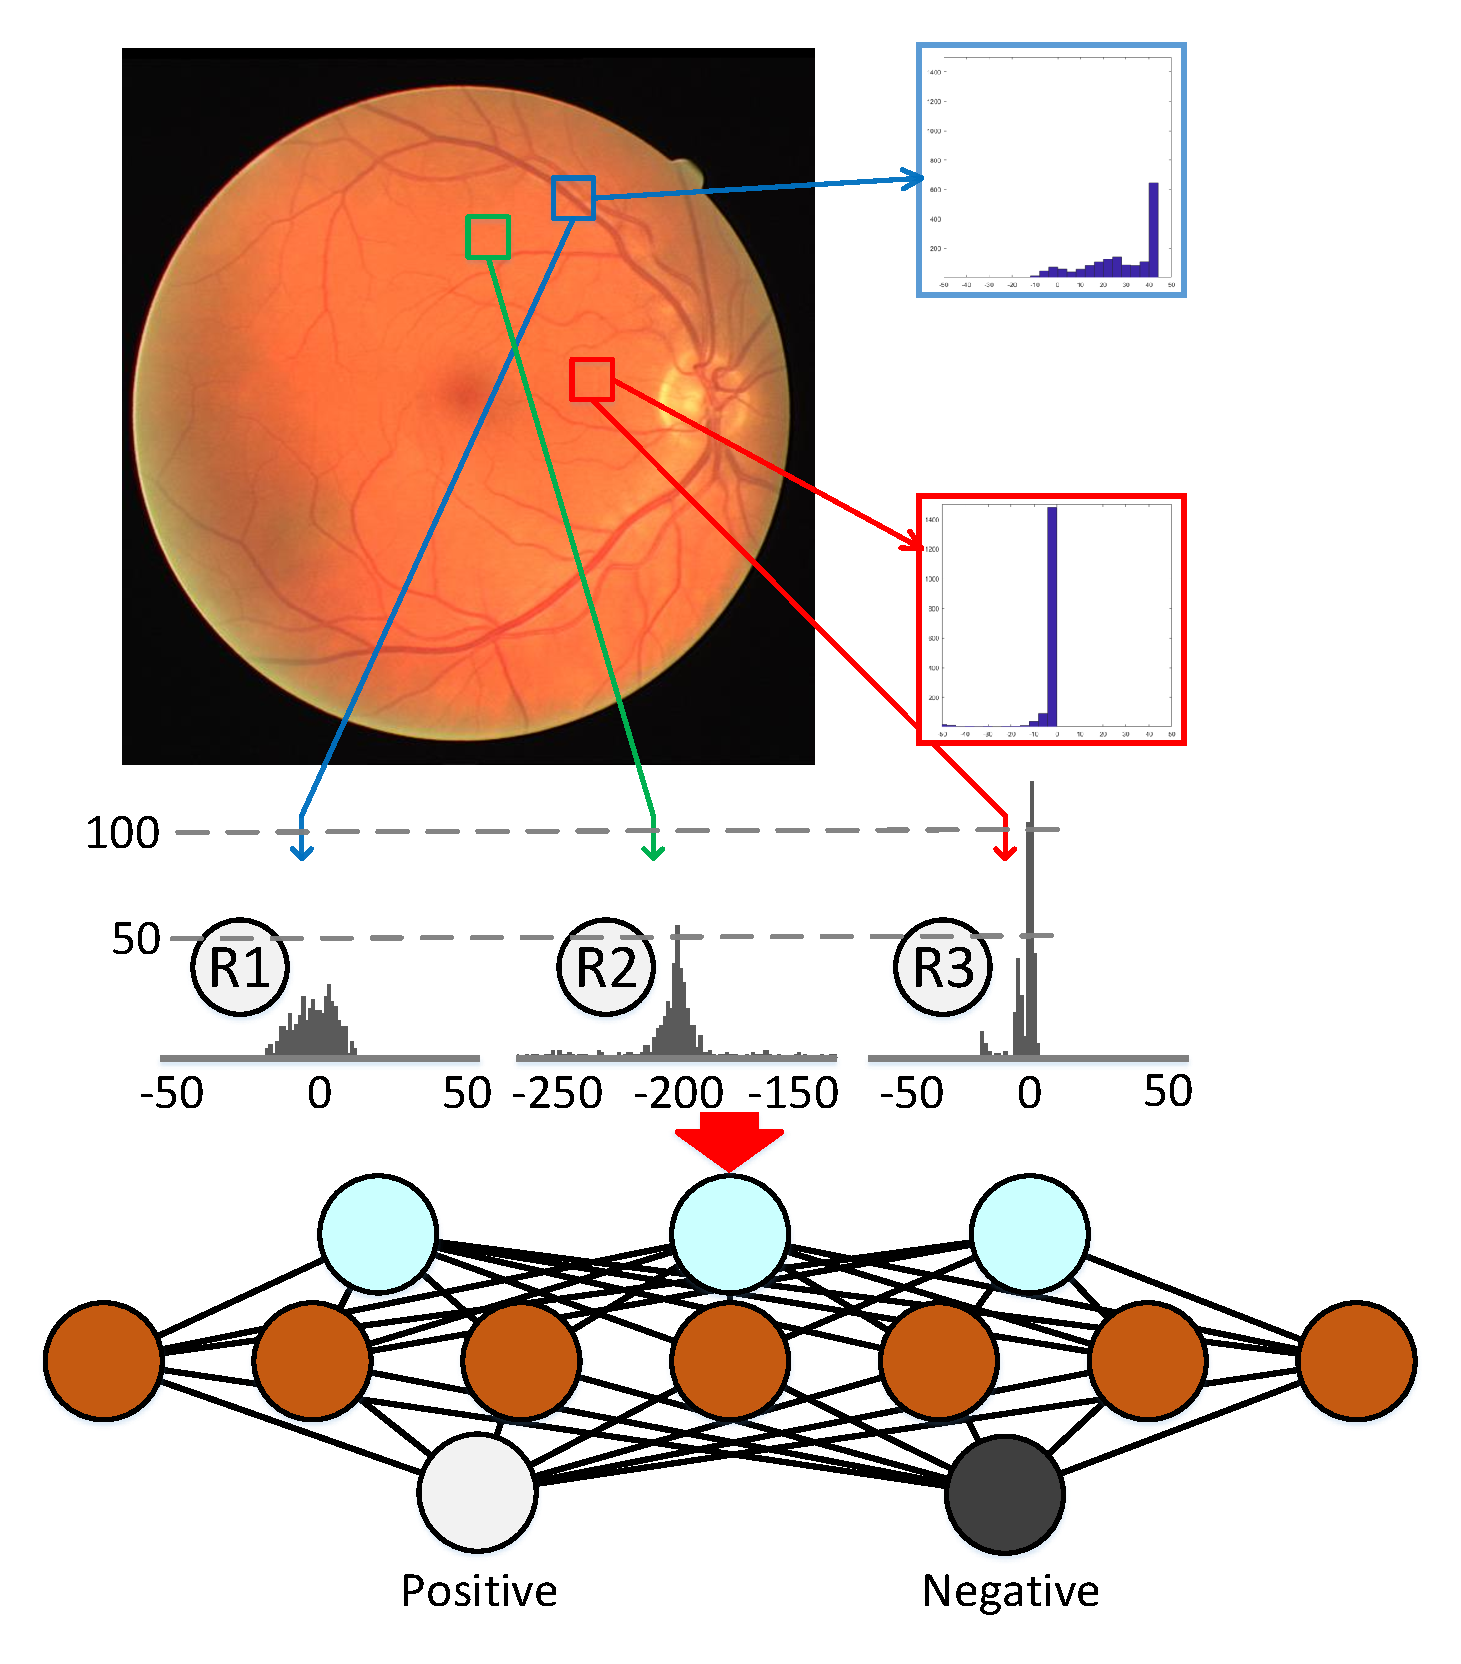
\includegraphics[width=0.5\textwidth]{figure/fig1.pdf}\\
    \label{fig1}
%  \vspace{-15pt}    % 对应高度2
  \caption{Deep distribution Learning.}
    \label{fig1}
%  \vspace{-15pt}    % 对应高度3
\end{wrapfigure}


% \begin{figure}[!h]
%     \centering
%     \includegraphics[width=0.5\textwidth]{../imgs/distribution.pdf}
%     \caption{Segmenting moving objects in freely moving camera.}
%     \label{fig_intro}
% \end{figure}
Motion is a powerful cue for image and scene segmentation in human visual system.
%
It has wide range of applications such as video monitoring, optical motion capturing and multimedia applications.
%
The human ability to detect, segment, analyze and understand motion is nearly instantaneous,
and work well in diversely complex scenes.
%such as the presence of multiple objects,
%dynamic background and even camouflage.
%
While there has been much recent progress related to motion, it still appears we are far from human capabilities.
%
Therefore,
as an essential and fundamental research topic related to motion of computer vision,
background subtraction has been attracting increasing attention in the recent years.

The main aim of background subtraction is to separate object with motion from the background in a video,
in which each pixel is classified into two classes, namely, foreground class which represents the moving objects,
and background class which corresponds to the background scenes.
%
Traditionally,
background is subtracted by the analysis of pixels' observations,
and plenty of previous work address the problem by approximating the distribution of observations via statistic model.
%
However,
due to the complexity and the diversity of natural scenes,
the distribution generated by pixels is so hard to be approximated by artificial model perfectly,
as shown in the \reffig{fig1}.

% background subtraction的本质
Essentially, background subtraction is the classification of pixels in a sequence of image frames,
typically under the assumption of a static camera,
wherein each pixel in a particular frame is classified as foreground or background by comparing its current measurement with historical observations.
%
When dealing with diverse and complex scenes,
it is a challening problem as the pixel measurements take the form of complex distributions for the pixels in both foreground and background.
%
For example,
as shown in the \text{R1}, \text{R2} and \text{R3} of \reffig{fig1},
the distributions of the pixel values in the pixels belonging to a dynamical background, moving objects and a static background are completely different,
and manually-tailored models have limited ability to cope with these contrasting distributions.
%
In this proposal,
we focus on learning the distribution automatically instead of devising the sophisticated model,
and deep learning network is naturally be selected to learn the distribution,
due to it is excellent learning ability shown recently years.

% extend 的distribution learning to high level
Moreover,
the distribution itself has a wide range of applications.
Therefore, the distribution learning can not only be used in background subtraction,
but also in some other research problems, such as tracking, object detection, or even some challenging problem outside of the computer vision,
in which tons of research work can be done.
%
Hence,
like the hierarchical features learned by deep learning network,
which work better than all these artificial features,
\textbf{is there any hierarchical representation of distribution implied which is not be discovered yet?}
%
\textbf{Will this high level distribution work better than the existed techniques, e.g. histogram, density estimation and so on, related to distribution?}
%
Solving this problem would be extremely interesting, which is the \textbf{main purpose of "\textcolor{red}{Deep} Distribution Learning".}

% 
% % is there any hierarchical representation of distribution can be learned like the features 
% 
% % 
% % 
% % it is naturally to utilize the learning network for learning the distribution,
% % 
% % 
% % 
% % 
% % and it is naturally to model the distribution of observations for analysis.
% % 
% % % XXX
% % To solve this problem,
% % we focus on learning the distribution by deep learning network for bakground subtraction,
% % with the motivation to let the deep learning network learns to automatically adapt to the disparate distributions encountered in different scenes.
% % % XXX
% % 
% % % 为什么spatio-temporal 没用
% % In addition, it is tempting to focus on the spatio-temporal inforamtion to learn,
% % however, the lack of groundth may hurt the robustness of approaches when it is used in another video.
% % %
% % Therefore, 
% % we insist that the distribution is similar for similar scenes,
% % which makes the network easier to learn general information for background subtraction in different scenes.
% % 
% % 运动物体是不可预测的,不知道什么时候会出来
% 
% % 因为其不可预测性,导致时序信息迁移性太差。
% 
% % 因为两个视频的运动物体出现时间不一样, 学到了第一个,第二个没用
% 
% % 而分布就没有这个问题,因此可以解决训练帧的问题
% 
% 
% \section*{Brief Summary of Existing Work}
% 
% In this section, we cover the progression of background subtraction algorithms over three sections.
% %
% In \refsec{rel_ta}, 
% traditional background subtraction methods are introduced.
% %
% Background subtraction based on earlier machine learning techniques are discussed in \refsec{rel_ml},
% %
% while recent deep learning methods for background subtraction are described in \refsec{rel_dl}.
% 
% \subsection{Traditional Algorithms}
% \label{rel_ta}
% % statistic model
% Traditionally background subtraction is done by modeling the variation of pixel intensities over time
% %
% %In this condition, large numbers of previous work (e.g. \cite{Barnich2011_2011_TIP}, \cite{1407887},
% %\cite{Zivkovic2004}, \cite{2004_TIP_1344037}, \cite{2009_TM_4796296},
% %\cite{Varadarajan2013}, \cite{2013_TPAMI_6678500}, \cite{2014_ICIP_7025664},
% %\cite{2014_CVPRW_6910016},  \cite{2016_NC_RAMIREZALONSO2016990},
% %\cite{LIANG20151374}, \cite{2015arXiv150502921B}, \cite{2015_ICME_7177419},
% %\cite{2015_TIP_6975239}, \cite{2017_TCSVT_7911235}) focus on the statistic
% %model.
% (e.g. \cite{Barnich2011_2011_TIP, 1407887,
% Zivkovic2004, 2004_TIP_1344037, 2009_TM_4796296,
% Varadarajan2013, 2013_TPAMI_6678500, 2014_ICIP_7025664,
% 2014_CVPRW_6910016, 2016_NC_RAMIREZALONSO2016990,
% LIANG20151374, 2015arXiv150502921B, 2015_ICME_7177419,
% 2015_TIP_6975239, 2017_TCSVT_7911235}).
% %Moreover,
% %Then, 
% %\cite{2017_TCSVT_7911235} XXX
% %      STGSR\cite{2017_TCSVT_7911235}
% %Background Subtraction using Spatio-Temporal Group Sparsity Recovery , we take
% %into account the group properties of foreground signals in both spatial and
% %temporal domains, and propose a greedy pursuit based method called
% %Spatio-Temporal Group Sparsity recovery, which prunes data residues in an
% %iterative process, according to both sparsity and group clustering priors,
% %rather than merely sparsity. Furthermore, a random strategy for background
% %dictionary learning is used to handle complex background variations, while
% %foreground-free training is not required.
% %
% In particular, 
% the Gaussian mixture model \cite{Zivkovic2004}
% is one of the more popular techniques for background subtraction \cite{Goyal2017},
% and numerous extensions of GMM have been proposed.
% %
% For example, Varadarajan et al.\ \cite{Varadarajan2013} modeled regions rather than pixels using a Gaussian distribution to represent neighbouring relationships.
% %
% %Likewise,
% Sriram et al.\ \cite{2015_PR_Varadarajan20153488} extend this through the use of expectation maximization.
% %
% In addition, there are also several algorithms that utilize kernel density estimation (e.g. \cite{Elgammal2000, han2004sequential, 2010_CVPR_Liao2010,
% 2012_TIP_6203582, 2012_ICSP_6491583}) as a substitute for Gaussians.
% %
% Recently, Haines et al.\ \cite{2014_TPAMI_6678500, 2012_ECCV_Haines2012} proposed the use of Dirichlet processes with Gaussian mixture models to analyze pixel distribution,
% while Chen et al.\ \cite{2017_TPAMI_Chen, 2014_ECCV_Chen2014} used Gaussian mixture models representing the vertices of spanning trees.
% %Besides the GMM \cite{Zivkovic2004}, there are also several algorithms focus on statistic model.
% %In addition to the GMM, Barnich et al.\ \cite{Barnich2009}, \cite{Barnich2011_2011_TIP} utilized the random strategy to describe the background,
% %and Tiefenbacher et al.\ \cite{2014_ICIP_7025664} proposed the proportional-integral-derivative controllers for background update.
% %%
% %Then, Graciela et al.\ \cite{2016_NC_RAMIREZALONSO2016990} reduced the false positive rates through a suspicious foreground analysis.
% %%
% %In addition, Liang et al.\ \cite{LIANG20151374} used a two-stage training framework to model the background,
% %which employs join histogram to screen the supporting pixels and optimizes the distribution of supporting pixels by spatial sampling.
% %  SuBSENSE
% %
% % Bianco et al.\ \cite{2015arXiv150502921B} combined several related algorithms by leveraging their individual peculiarities,
% % and the genetic programming is used to combine the output, and achieves well performances in severally different scenes.
% 
% Besides GMMs, there are also several other recent advances (e.g. \cite{2015_TIP_6975239, 2017_TFS_7468482, 2017_TIP_7904604, 2017_TCSVT_7938679, 2017_TCSVT_7434630, 2016_TIP_7539354}) in background subtraction.
% %
% Charles et al.\ \cite{2015_TIP_6975239} utilized temporal binary features and color information for background subtraction.
% %
% Moreover,
% inspired by the traditional codebook algorithm \cite{Kim2004},
% they also utilized word dictionaries for background subtraction \cite{2016_TIP_7539354}.
% %
% Zeng et al.\ \cite{2017_TFS_7468482} proposed the use of a histogram based on strong uniform fuzzy partitions,
% where the threshold for background segmentation is set adaptively according to the shape of the histogram.
% %
% Sajid et al.\ \cite{2017_TIP_7904604} proposed a universal multi-mode system
% % which improves the performance by several innovative mechanisms, such as the multiple color spaces and mega-pixels.
% that merged pixels together to form what the authors called mega-pixels, which aided the denoising of foreground masks in different RGB and YCbCr color spaces.
% % , model update, pixel classification, and the use of multiple color space.
% %
% % trational method R-PCA 
% Javed et al.\ \cite{2017_TIP_8017547} proposed a robust principal component analysis framework,
% which incorporates spatial and temporal sparse subspaces.
% %proposed the robust principal component,
% % incorporate the spatial and temporal sparse subspace clustering into the robust principal component analysis (RPCA) framework.
% %
% Finally,
% Huynh et al.\ \cite{2017_TCSVT_7434630} identified moving pixels for comparing current and background frames,
% %captured the difference between background and current frame by identifying the motion pixels,
% while Jiang et al.\ \cite{2017_TCSVT_7938679} utilized a weighted-sample method to rapidly adapt to changing scenarios.
% 
% However, such hand-crafted models do not work effectively when applied to a wide range of scene categories.
% %
% For example, 
% GMM-based algorithms suffer from performance degradation in scenes with high complexity \cite{2017_TIP_8017547},
% where the distributions of pixels are too complex to be described even by several Gaussian components.
% %
% 
% % machine learning method
% \subsection{Algorithms based on Machine Learning}
% \label{rel_ml}
% Besides traditional algorithms,
% there are also several background subtraction methods that utilize machine learning,
% %these are several work focus on using machine learning to handle the background subtraction.
% %
% commonly involving support vector machines (SVM) and Bayesian methods.
% %
% Lin et al.\ \cite{2002_ICIP_1039116} proposed using a probabilistic SVM for background initialization,
% %
% Cheng et al.\ \cite{2009_ICCV_5459454} accommodated spatial interactions by minimizing a risk functional generalization of the one class SVM,
% and Han et al.\ \cite{2012_TPAMI_Han2012} utilized density-based features as the input to an SVM classifier.
% %
% Zhang et al.\ \cite{2014_ICME_6890245}, \cite{2017_TM_7920340} proposed an imbalance compensation mechanism for use with bilayer modeling and
% Bayesian classification.
% %
% Culibrk et al.\ \cite{2007_TNN_4359175} constructed an unsupervised Bayesian classifier for background modeling and subtraction using a neural network architecture.
% %
% The novel subspaces learning method proposed by Zhou et al.\ \cite{2013_TPAMI_6216381}, in which
% %
% a sequence of regular video
% bricks is extracted, poses the background modeling problem as pursuing a subspace representation for
% video bricks while adapting to scene variation.
% 
% In addition, there is also related work employing neural networks for background subtraction.
% %
% Gregorio et al.\ \cite{2011_ICME_6012085, 6910014} proposed a weightless neural network for dynamically adapting to background change, while
% %
% Maddalena et al.\ \cite{2008_TIP_4527178, 2012_CVPRW_6238922} proposed having background models be automatically generated through a self-organizing network, 
% which appears to work well in several scenes containing gradual illumination variation and camouflage.
% %
% %Gregorio et al.\ \cite{6910014} also utilized the weightless neural network for background subtraction,
% %which can dynamically adapt to background change. 
% %
% %The main difference between our proposed approach and these previous methods is the use of deep learning.
% %
% %As mentioned previously, the traditional machine learning classifiers are not strong enough for handling numerous kinds of natural scenes,
% %since the diversity and the complexity of natural scenes.
% %
% %But in this work, the strong learning ability guarantees the performances of proposed approach in diversity natural scenes.
% %
% 
% \subsection{Algorithms based on Deep Learning}
% \label{rel_dl}
% %Hence, there are several excellent works (e.g. \cite{2016_PRL_Wang}, \cite{2016_IWSSIP_7502717}, \cite{2017arXiv170201731B}) utilized the deep learning for background %subtraction recently.
% Unsurprisingly, recent background subtraction methods have embraced deep learning.
% %
% Wang et al.\ \cite{2016_PRL_Wang} used a cross-entropy loss function for training a multi-scale CNN to learn the background of a current scene, using the full image as input.
% %
% Braham et al.\ \cite{2016_IWSSIP_7502717} employed a deep network to evaluate the difference between current frames and a background image,
% the latter being computed as the temporal median across multiple frames.
% %
% In both these works, a large number of frames is needed in the training phase to achieve accurate segmentation of moving objects.
% %Unfortunately, similar to the Wang et al's work \cite{2016_PRL_Wang}, it needs numbers of frames for training to let the algorithm segment moving objects successfully.
% %
% % Moreover, since the background is captured from the temporal median, the background image has limited ability to describe the dynamic background.
% %
% A more robust background model algorithm was proposed by Babaee et al.\ \cite{2017arXiv170201731B} for background extraction,
% with a network used for subtracting the background from the current image.
% 
% %What the network learned is the main difference between proposed approach and these previously deep learning algorithms.
% %%
% %Both of these work used the deep learning network in the comparison between background image and current frames.
% %%
% %What the network learned is a representation of background image in these previous work.
% %%
% %It ignore the fact that a single background image can not describe the complex natural scenes completely, such as the dynamic background.
% %%
% 
% % In contrast, our proposed method departs from the conventional approach of creating an explicit representation of the background scene, which we expect
% % will face considerable difficulty in modeling a dynamic and complex background well.
% % Instead we focus on the more fundamental concept underlying background subtraction, 
% % which is the classification of pixels in a time sequence \cite{Barnich2011_2011_TIP},
% % based on network-learned discriminative features that act directly on the distribution of pixels across time.
% %
% %The network learned the distribution of pixels' observations and the difference between distributions in pixels belong to foreground and background.
% %
% %Moreover, each pixel can provide an instance for training,
% %and large numbers of training instances can be captured with only one groundtruth.
% %
% %Therefore, our DPDL model is effective even with only one groundtruth frame,
% %which is one of the advantage of proposed approached compared with these existed deep learning method.
% 
% 
% 
% \section*{What you Plan To Do}
% There are fives sub-topics for deep distribution learning.
% The first one "Temporal Distribution Learning" have done in one of our previous work at this year (2018).
% For class 608,
% we will only focus on the second topic (Spatio-Temporal Distribution Learning),
% and the remaining topics will be finished after the class 608.
% 
% \begin{itemize}
%     \item Temporal Distribution Learning:
%         Learn the distribution of temporal observations in a pixel, then classify if the pixel is foreground or background according to the distribution learned.
%     \item Spatio-Temporal Distribution Learning:
%         Incorporate the neighbouring information of pixels to improve the robustness and the efficiency of our background subtraction algorithm.
%     \item Distribution Learning Layer:
%         Devise a specific layer to learn the distribution.
%     \item High Level Distribution Representation:
%         Try to figure out what is the high level representation of distribution, what is the distribution of distribution.
%     \item Deep Distribution Learning for General Problem:
%         Extend the Deep Distribution Learning to other problems, instead of only used in background subtraction.
% \end{itemize}
% 
% % , for class 608, we will only focus on the second topic.
% % The 
% % 
% % 
% % Learn the distribution via deep network
% % Force the network to learn the distribution
% % 
% % Devise specific layer for learning.
% % 
% % Incorporate the spatial information in the learning procedure to improve the robustness of learning process.
% % 
% % The "Deep" distribution:
% % What is the distribution of distribution is? Is there some new thing comes from multiple distribution,
% % a hierarchical representation of distribution.
% % 
% % % 即便没有更高级别的表示,可以学到distribution 也足够了,至少比核密度估计要好
% % The deep distribution network?
% % 
% % Deep distribution for background subtraction
% % 
% % Deep distribution for general problem
% % Besides the background subtraction, there is many other problems can be solved by distribution learning
% % 
% % Learning the 
% 
% \section*{How You Plan to Implement Your Ideas}
% For the class 608, we will only focus on the second sub-topics, the Spatio-Temporal Distribution Learning.
% The potential architecture for learning the spatio-temporal distribution is shown as \reffig{fig2},
% in which there are two networks to learn the distribution implied in spatial information and temporal information respectively.
% In particular,
% the distribution information implied in temporal observations of pixel is described by a feature,
% which is used as the input of network to force the network focus on the distribution information.
% %
% Then, the output of network is incorporated with the distribution information from the spatial observations of pixel 
% and used as the input of the second network.
% %
% Benefited from the strong learning ability of deep learning network,
% the performance of this potential architecture should be well.
% 
% \begin{figure*}[!t]	% FIGURE: figure/fig1 
% \centering
% 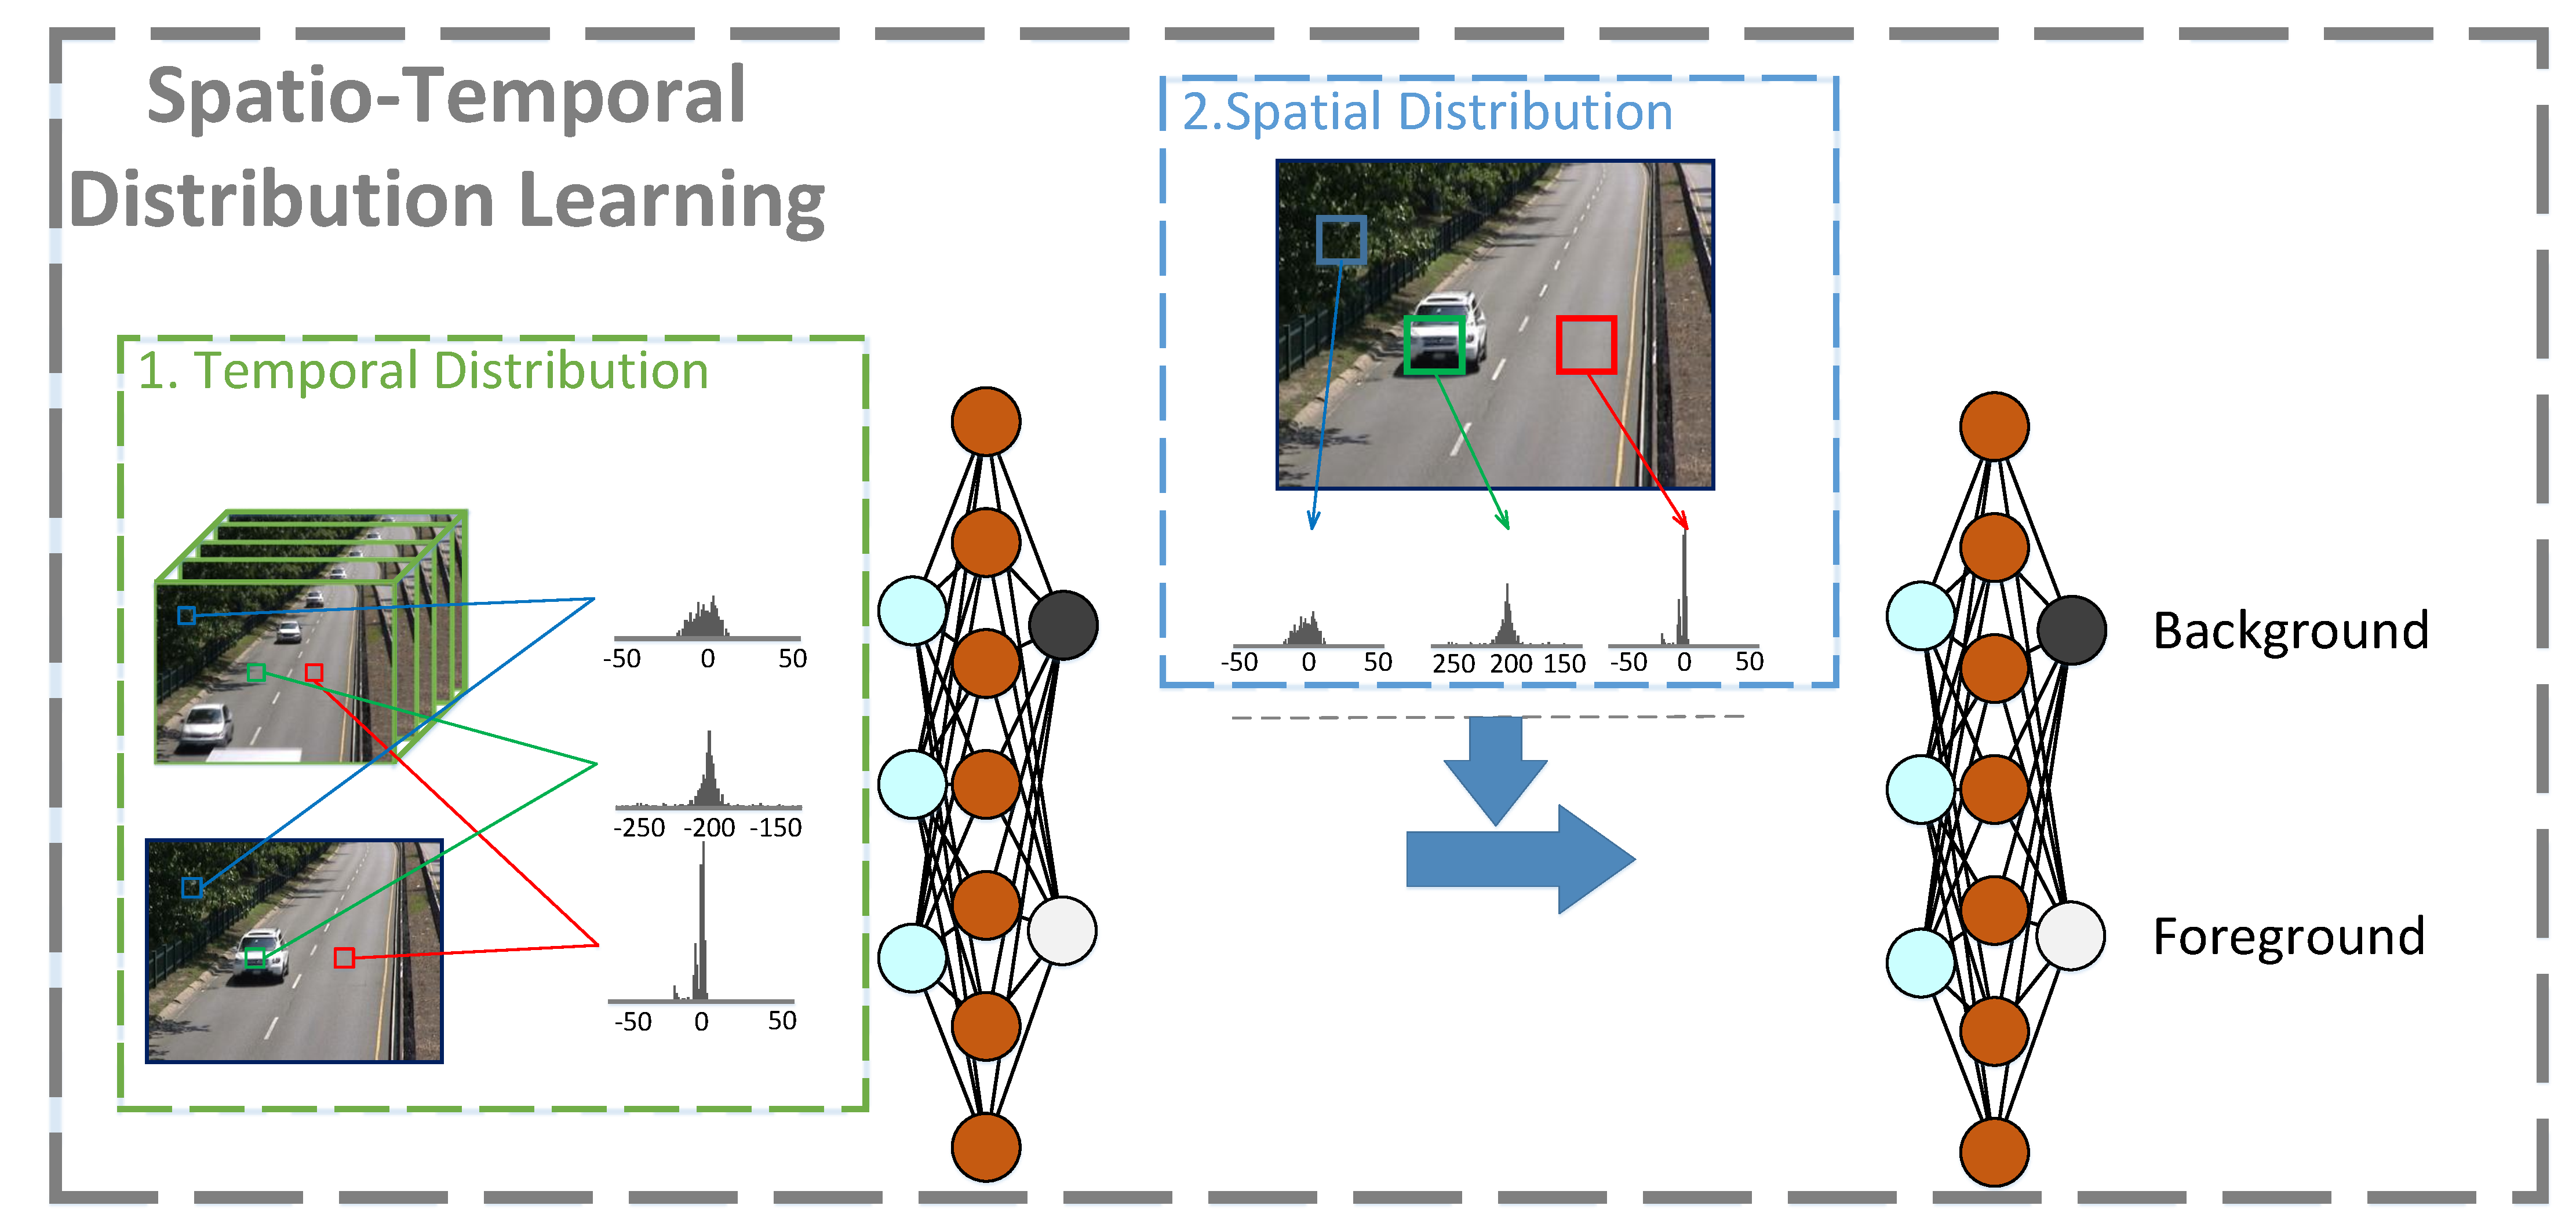
\includegraphics[width=\textwidth]{figure/fig2}
% \DeclareGraphicsExtensions.
% 	\caption{The potential architecture of Spatio-Temporal Distribution Learning Network.}
%     \label{fig2}
% \end{figure*}
% 
% 
% 
% 
% 
% 
% % \begin{itemize}
% %     \item Temporal Distribution Learning:
% %     \item Spatio-Temporal Distribution Learning:
% %     \item Distribution Learning Layer:
% %     \item High Level Distribution Representation:
% %     \item Deep Distribution Learning for General Problem:
% % \end{itemize}
% 
% % Random permutation to force the network learn the distribution
% % 
% % Learn the distribution from spatial information
% % 
% % Figure out what the layer learned, then devise a specific layer to generate the same result.
% % 
% % Tried if there is a high level representation of distribution,
% % can we proposed a network to learn it.
% % 
% % There are other problems can be solved by distribution learning
% 
% \section*{Timeline for Deep Distribution}
%   \begin{tikzpicture}[x=4mm,y=7mm]
%     % draw the grid
%     \draw[help lines] (0,0) grid[step=1] (36,7);
%     \draw (0,0) grid[xstep=2,ystep=7] (36,7);
%     % put months and years under the x-axis
%     \foreach[count=\a] \aa in {2018,...,2020} {
%       \draw[gray] (12*\a-12,0) -- +(0,-7mm) node[pos=.5, below right, inner sep=1pt]{$\aa$};
%       \foreach[count=\m] \mm in {J,F,M,A,M,J,J,A,S,O,N,D}
%         \node[font=\tiny,below,gray] at (12*\a+\m-12.5,0) {\mm};
%     }
% 
%     % plot the data
% 
%       \chronoperiode{TDL(Done)}{2018}{1}{2018}{7}{1}{level1}
%       \chronoperiode{STDL}{2018}{9}{2018}{13}{2}{cyan}
%       \chronoperiode{DLL}{2018}{12}{2019}{6}{3}{brightube}
%       \chronoperiode{HLDR}{2019}{4}{2019}{11}{4}{fuchsia}
%       \chronoperiode{DDLGP}{2019}{10}{2020}{10}{5}{heliotrope}
% %      \chronoperiode{test}{2018}{4}{2019}{10}{1}{olive}
% %      \chronoperiode{Incorporating spatial information}{2018}{10}{2019}{10}{2}{cyan}
%   \end{tikzpicture}
% 
%   \begin{itemize}
%     \item    TDL: Temporal Distribution Learning.
%     \item    STDL: Spatio-Temporal Distribution Learning.
%     \item    DLL: Distribution Learning Layer.
%     \item    HLDR: High Level Distribution Representation.
%     \item    DDLGP: Deep Distribution Learning for General Problem.
%   \end{itemize}
% 
% 
% 
% \section*{Timeline for Spatio-Temporal Distribution Learning(Class 608)}
%   \begin{tikzpicture}[x=9mm,y=7mm]
%     % draw the grid
%     \draw[help lines] (0,0) grid[step=1] (16,7);
%     \draw (0,0) grid[xstep=2,ystep=7] (12,7);
%     % put months and years under the x-axis
%     \foreach[count=\a] \aa in {9,...,12} {
%       \draw[gray] (4*\a-4,0) -- +(0,-7mm) node[pos=.5, below right, inner sep=1pt]{2018. $\aa$};
%       \foreach[count=\m] \mm in {Week1, Week2, Week3, Week4}
%         \node[font=\tiny,below,gray] at (4*\a+\m-4.5,0) {\mm};
%     }
% 
%     % plot the data
% 
%       \chronoperiode{Review of Existed Work}{2018}{1}{2018}{6}{1}{level1}
%       \chronoperiode{Experiments}{2018}{5}{2019}{1}{2}{cyan}
%       \chronoperiode{Paper Writing}{2018}{6}{2019}{5}{3}{brightube}
% %      \chronoperiode{HLDR}{2019}{4}{2019}{11}{4}{fuchsia}
% %      \chronoperiode{test}{2018}{4}{2019}{10}{1}{olive}
% %      \chronoperiode{Incorporating spatial information}{2018}{10}{2019}{10}{2}{cyan}
%   \end{tikzpicture}
% 
% %   \begin{itemize}
% %     \item    TDL: Temporal Distribution Learning.
% %     \item    STDL: Spatio-Temporal Distribution Learning.
% %     \item    DLL: Distribution Learning Layer.
% %     \item    HLDR: High Level Distribution Representation.
% %     \item    DDLGP: Deep Distribution Learning for General Problem.
% %   \end{itemize}
% 


\small
\bibliographystyle{unsrt}
% \bibliographystyle{plain}
\bibliography{ref.bib}  




\end{document}
